\chapter{DUNE Physics}
\label{ch:exec-summ-physics}

DUNE will address fundamental questions key to our understanding of the universe. These include:
\begin{itemize}
   \item {\bf What is the origin of the matter-antimatter asymmetry in the universe?} Immediately after
                    the Big Bang, matter and antimatter were created equally, but now matter dominates.
                    By studying the properties of neutrino and antineutrino oscillations, LBNF/DUNE 
                    will pursue the current most promising avenue for understanding this asymmetry.
   \item {\bf What are the fundamental underlying symmetries of the universe?} The patterns of mixings and masses between the particles of the Standard Model is not understood. By making precise measurements of the mixing between the neutrinos and the ordering of neutrino masses and comparing these with the quark sector, LNBF/DUNE could reveal new underlying symmetries of the universe.
  \item{\bf  Is there a Grand Unified Theory of the Universe?} Results from a range of experiments suggest that the
                 physical forces observed today were unified into one force at the birth of the universe.
                Grand Unified Theories (GUTs), which attempt to describe the unification of forces,
                predict that protons should decay, a process that has never been observed. DUNE will 
                search for proton decay in the range of proton lifetimes predicted by a wide range of GUT models.
   \item{\bf How do supernovae explode and what new physics will we learn from a neutrino burst?}
   Many of the heavy elements that are the key components of life were created in the super-hot cores of collapsing stars. DUNE would be able to detect the neutrino bursts from core-collapse supernovae within our galaxy (should any occur). Measurements of the time, flavor and energy structure of the neutrino burst will be critical for understanding the dynamics of this important astrophysical phenomenon, as well as bringing information on neutrino properties and other particle physics.
\end{itemize}

%%%%%%%%%%%%%%%%%%%%%%%%%%%%%%%%%%%%%%%%%%%%%%%%%%%%%%%%%%%%%%%%%%%%
\section{Introduction: Scientific Goals}
\label{sec:exec-summ-physics-goals}


The DUNE scientific objectives are categorized into: the \textit{primary science program}, addressing the key science questions 
highlighted by the particle physics project prioritization panel (P5); 
a high-priority \textit{ancillary science program} that is 
enabled by the construction of LBNF and DUNE; and \textit{additional scientific objectives}, that may require further developments 
of the LArTPC technology. A detailed description of the physics objectives of DUNE is provided in \href{http://arxiv.org/abs/1512.06148}{Volume 2 of the DUNE Conceptual Design Report}.

%%%%%%%%%%%%%%%%%%%%%%%%%%%%
\subsection{The Primary Science Program}

The primary science program of LBNF/DUNE  focuses on fundamental open questions in neutrino and astroparticle physics: 
\begin{itemize}
  \item precision measurements of the parameters that govern $\nu_{\mu} \rightarrow \nu_\text{e}$ and
           $\overline{\nu}_{\mu} \rightarrow \overline{\nu}_\text{e}$ oscillations with the goal of
  \subitem -- measuring the charge-parity (CP) violating phase $\delta_\text{CP}$, where a value differing from zero or $\pi$ would represent the discovery of CP violation in the leptonic sector, providing a possible explanation for the matter-antimatter asymmetry in the universe;
  \subitem -- determining the neutrino mass ordering (the sign of $\Delta m^2_{31} \equiv m_3^2-m_1^2$), often referred to as the neutrino \textit{mass hierarchy}; and
  \subitem -- precision tests of the three-flavor neutrino oscillation paradigm through studies of muon neutrino disappearance 
    and electron neutrino appearance in both $\nu_\mu$ and $\overline{\nu}_{\mu}$ beams, including the 
    measurement of the mixing angle $\theta_{23}$ and the determination of the octant in which this angle lies.
    \item search for proton decay in several important decay modes, for example $\text{p}\rightarrow\text{K}^+\overline{\nu}$, where the observation of proton decay would represent a ground-breaking discovery in physics, providing a portal to Grand Unification of the forces; and
    \item detection and measurement of the $\nu_\text{e}$ flux from a core-collapse supernova within our galaxy, should one occur during the lifetime of the DUNE experiment.
\end{itemize}

%%%%%%%%%%%%%%%%%%%%%%%%%%%%%
\subsection{The Ancillary Science Program}

The intense neutrino beam from LBNF, the massive DUNE LArTPC far detector and the high-resolution
  DUNE near detector provide a rich ancillary science program, beyond the primary mission of the experiment. The ancillary science program includes
\begin{itemize}
     \item other accelerator-based neutrino flavor transition measurements with sensitivity to Beyond Standard Model (BSM) physics, such as: non-standard interactions (NSIs); the search for sterile neutrinos at both the near and far sites;
 and measurements of tau neutrino appearance;
     \item measurements of neutrino oscillation phenomena using atmospheric neutrinos;
     \item a rich neutrino interaction physics program utilizing the DUNE near detector, including: a wide-range of measurements of neutrino cross sections; studies of nuclear effects, including neutrino final-state interactions; measurements of the structure of nucleons; and  measurement of $\sin^2\theta_\text{W}$; and
     \item  the search for signatures of dark matter.
\end{itemize} 

Furthermore, a number of previous breakthroughs in particle physics have been serendipitous, in the sense that they were beyond the
original scientific objectives of an experiment. The intense LBNF neutrino beam and novel capabilities for both 
the DUNE near and far detectors will probe new regions of parameter space for both the accelerator-based and astrophysical frontiers, 
providing the opportunity for discoveries that are not currently anticipated.



%%%%%%%%%%%%%%%%%%%%%%%%%%%%%%%%%%%%%%%%%%%%%%%%%%%%%%%%%%%%%%%%%%%%
\section{Long-Baseline Neutrino Oscillation physics program}
\label{sec:exec-summ-physics-osc}

\fixme{6 pages}
Precision neutrino oscillation measurements lie at the heart of the DUNE scientific program.
The \SIadj{1300}{\km} baseline, coupled with the wide-band
high-intensity neutrino beam from LBNF, establishes one of DUNE's key
strengths, namely sensitivity to the matter effect. This effect leads to a
discrete asymmetry in the \numu $\to$ \nue versus \anumu $\to$ \anue
oscillation probabilities, the sign of which depends on the presently
unknown mass hierarchy (MH).  At \SI{1300}{\km} the asymmetry,
\begin{equation}
\mathcal{A} = \frac{ P(\nu_\mu \rightarrow \nu_e)-P(\bar{\nu}_\mu \rightarrow \bar{\nu}_e)}{P(\nu_\mu \rightarrow \nu_e)+P(\bar{\nu}_\mu \rightarrow \bar{\nu}_e)}
\end{equation}
is approximately $\pm 40\%$ in the region of the peak flux in the
absence of CP-violating effects. This is larger than the maximal
possible CP-violating asymmetry associated with the CP-violating
phase, \deltacp, of the three-flavor PMNS mixing matrix in the region of
the peak flux. The CP asymmetry is larger in the energy regions below the peak
flux while the matter asymmetry is smaller. As a result, the LBNF
wide-band beam will allow unambiguous determination of both the MH and
\deltacp with high confidence \textit{within the same experiment}, i.e., DUNE. 
The DUNE science reach is described in detail in %\volphys, 
where it is presented 
in terms of  exposure expressed in units of \ktMWyr{}.

For instance, seven years of data
(\num{3.5} years in neutrino mode plus \num{3.5} years in antineutrino
mode\footnote{unless otherwise stated, the results presented in the CDR assume equal running in neutrino and antineutrino mode.}) with a \ktadj{40} detector and a \MWadj{1.07} beam (based on a \GeVadj{80} primary proton beam) correspond to an
exposure of \SI{300}~\ktMWyr. 

The DUNE far detector will be built as four \ktadj{10} modules, which will
come online sequentially over the course of several years, as described in Chapter~\ref{ch:project-overview}. 
This staged program enables an early scientific output from DUNE, 
initially focused on the observation of natural
sources of neutrinos, searches for nucleon decays and 
measurements of backgrounds. 
About a year after commissioning the first detector module, 
the LBNF neutrino
beam at Fermilab will  
begin sending neutrinos over the \kmadj{1300}
baseline, commencing the LBL oscillation physics program with a beam power of up to \SI{1.2}\MW{}. 
Prior to the operation of the near detector (ND), which
is likely to start after the initial beam running, the early physics program
will be statistically limited. However, the constraints from comparison of the $\nu_\mu$
disappearance spectrum with that from $\nu_e$ appearance mitigate, in part,
the absence of a direct flux measurement from the ND. Subsequently, the ND
measurements will provide powerful constraints on the beam flux, providing the
necessary control of systematic uncertainties for the full exploitation of LBNF/DUNE. 


The evolution of the projected DUNE sensitivities as a function of real time
(for the first \num{15} years of operation) was estimated based on an assumed deployment plan
with the following assumptions:

\begin{itemize}
\item Year 1: \SI{10}\kt{} far detector mass, \MWadj{1.07} \GeVadj{80}
  proton beam with $1.47 \times 10^{21}$ protons-on-target per year 
  and no ND
%%%(assume \num{5}\% signal systematic)
\item Year 2: Addition of the second \ktadj{10} far detector module, for a total far detector mass of
  \SI{20}\kt
\item Year 3: Addition of the third \ktadj{10} far detector module, for a total far detector mass of
  \SI{30}\kt, and first constraints from the preliminary ND data analysis
%%%%  (assume \num{3}\% signal systematic)
\item Year 4: Addition of the fourth \ktadj{10} far detector module, for a total far detector mass of
  \SI{40}\kt
\item Year 5: Inclusion of constraints from a full ND data analysis
%%%%(assume  \num{2}\% signal systematic)
 \item Year 7: Upgrade of beam power to \SI{2.14}{\MW} for a \SIadj{80}{\GeV}
  proton beam
\end{itemize}
The staging of the detectors and facility in the resource-loaded schedule leads to a similar
evolution of physics sensitivity as a function of time.
In addition, it was assumed that the knowledge from the near detector can be
retroactively applied to previous data sets, such that each
improvement in the knowledge of systematic uncertainties~\footnote{A
  detailed discussion of the systematic uncertainties assumed, given a
  near detector, is presented in %\volphys. 
  For studies without a near
  detector an uncertainty of 10\% is assumed on the unoscillated flux
  at the far detector based on the current performance of the NuMI
  beam simulation, with uncertainties on physics backgrounds $\geq
  10\%$ depending on the background.} is applied to the full exposure
up to that point.

%%%%%%%%%%%%%%%%%%%%%%%%%%%%%%%%%
\subsection{Mass Hierarchy and CP Violation}
\label{sec:exec-summ-physics-mh-cpv}

\fixme{3 pages, spectra, numbers of events, sensitivities, plots}
\fixme{this heading for TP was not in CDR; Anne placed it here 19/2/18}

The discriminating power between the two MH hypotheses is quantified
by the difference, denoted $\Delta \chi^2$, between the
$-2\log{\cal L}$ values calculated for the normal and inverted
hierarchies. As the sensitivity depends on the true value of the unknown
CP-violating phase, \deltacp, all possible values of \deltacp are
considered\footnote{For the case of the MH determination, the usual
  association of this test statistic with a $\chi^2$ distribution for
  one degree of freedom is incorrect; additionally the assumption of a
  Gaussian probability density 
  implicit in this notation is not exact.  The discussion in Chapter~3
  of %\volphys{} 
  provides a brief description of the statistical
  considerations.}.  In terms of this test statistic, the MH
sensitivity of DUNE with an exposure of \SI{300}~\ktMWyr{} is
illustrated in Figure~\ref{fig:mhexec} for the case of normal
hierarchy and the current best-fit value of \sinst{23} = 0.45. 
For this exposure, the DUNE determination of the MH will be definitive for
the overwhelming majority of the  \deltacp and \sinst{23} parameter space.
Even for unfavorable combinations of the parameters, a statistically
ambiguous outcome is highly unlikely.  
\begin{dunefigure}[Summary of mass hierarchy sensitivities]{mhexec}{The
    square root of the mass hierarchy discrimination metric $\Delta
    \chi^2$ is plotted as a function of the unknown value of \deltacp
    for an exposure of \SI{300}~\ktMWyr{}  
    (left).  The minimum significance
    --- the lowest point on the curve on the left --- with which the mass
    hierarchy can be determined for all values of \deltacp as a
    function of years of running under the staging plan described in the text (right).
    The shaded regions represent the range in sensitivity corresponding to
    the different beam design parameters.}
%\includegraphics[width=0.49\textwidth]{mh_300ktmwyear}
%\includegraphics[width=0.49\textwidth]{mh_exp_staging15yr}
\label{fig:mhexec}
\end{dunefigure}


Figure~\ref{fig:mhexec} shows the evolution of the sensitivity to the MH determination as a function
of years of operation, for the least favorable scenario, corresponding to the case in which the MH asymmetry is
maximally offset by the leptonic CP asymmetry. For the reference design beam an exposure of \SI{400}~\ktMWyr{}  
(which corresponds to \num{8.5} years of operation) 
is required to distinguish
between normal and inverted hierarchy with $|\Delta \chi^2| =
\overline{|\Delta \chi^2|} = 25$.  This corresponds to a $\geq
99.9996\%$ probability of determining the correct hierarchy. 
Investments in a more capable target and horn focusing system can
lower the exposure needed to reach this level of sensitivity from
\SI{400}~\ktMWyr{} to around \SI{230}~\ktMWyr{} (\num{6.5} years of
running in the example staging plan). The dependence of the mass
hierarchy sensitivity on systematics is still under evaluation, but
current studies indicate a only weak dependence on the assumptions for 
the achievable systematic uncertainties. This indicates that a measurement of the unknown
neutrino mass hierarchy with very high precision can be carried out
during the first few years of operation with an optimized beamline
design, discussed in Section~\ref{v1ch:tech-designs:beam-strategy} and  %\vollbnf.
Concurrent analysis of the corresponding atmospheric-neutrino
samples in an underground detector will improve the precision and
speed with which the MH is resolved.


DUNE will search for CP violation using the \numu to \nue and \anumu
to \anue oscillation channels, with two objectives.  First, DUNE aims
to observe a signal for leptonic CP violation independent of the
underlying nature of neutrino oscillation phenomenology. Such a signal
will be observable in comparisons of $\nu_\mu \rightarrow \nu_e$ and
$\bar{\nu}_{\mu} \rightarrow \bar{\nu}_e$ oscillations of the LBNF
beam neutrinos in a wide range of neutrino energies over the
\SIadj{1300}{\km} baseline.
Second,
DUNE aims to make a precise determination of the value of \deltacp
within the context of the standard three-flavor mixing scenario
described by the PMNS neutrino mixing matrix. Together, the pursuit of
these two goals provides a thorough test of the standard three-flavor
scenario.

\begin{dunefigure}[CP-violation sensitivity and $\delta_{\rm CP}$
  resolution as a function of exposure]{execsummaryCP}{The
    significance with which CP violation can be determined for 75\% of
    \deltacp values (left) and the expected 1$\sigma$ resolution
    (right) as a function of exposure in years using the proposed
    staging plan outlined in this chapter. The shaded regions
    represent the range in sensitivity due to potential variations in
    the beam design. The plots assume normal mass hierarchy.}
%\includegraphics[width=0.49\textwidth]{cpv75_exp_staging15yr}
 %\includegraphics[width=0.49\textwidth]{dcp_exp_staging.pdf}
\end{dunefigure}
%
Figure~\ref{fig:execsummaryCP} shows, as a function of time, the
expected sensitivity to CP violation expressed as the minimum significance
with which CP violation can be determined for 75\% of
\deltacp values.
Also shown is the 1$\sigma$ resolution for \deltacp as a
function of time for $\delta_{\rm CP}=0$ (no CP violation) and
$\delta_{\rm CP}=90^\circ$ (maximal CP violation). In both figures the staging scenario
described above was assumed.  The exposure required to measure
$\delta_{\rm CP} = 0 $ with a precision better than $10^\circ$ ranges
from 290 to \SI{450}~\ktMWyr{} depending on the beam design.
A full-scope LBNF/DUNE operating with multi-megawatt 
beam power can eventually achieve a precision 
comparable to the current precision on the CP phase in the
CKM matrix in the quark sector (5\%).

Table~\ref{tab:execosctable} summarizes the exposures needed to
achieve specific oscillation physics milestones, calculated 
for the current best-fit values of the known neutrino mixing parameters. 
Values for both the reference beam design and the optimized beamline design are shown.
For example, to reach $3\sigma$ sensitivity 
for 75\% of the range of \deltacp, a
DUNE exposure in the range of \num{850} to \SI{1320}~\ktMWyr{} is needed
for the optimized and reference beamline designs. 
Changes in the assumed value of
$\theta_{23}$ impact CP-violation and MH sensitivities the
most (discussed in %\volphys) 
and can either reduce or increase the 
discovery potential for CP violation. To reach this level of sensitivity 
a highly capable near neutrino detector is required to control systematic uncertainties at a level lower than
the statistical uncertainties in the far detector. No experiment can provide coverage at 100\% of
\deltacp values, since CP-violating effects vanish as \mdeltacp to 0
or $\pi$. Potential improvements in beamline geometry, focusing and target element designs
can significantly lower the exposure required for CP violation
discovery potential.  Several such potential improvements are discussed
in CDR %\volphys and \vollbnf. 
 %
\begin{dunetable}[Required exposures to reach oscillation physics
  milestones]{lcc}{execosctable}{The exposure in mass (kt) $\times$ proton beam power
    (MW) $\times$ time (years) needed to reach certain oscillation physics
    milestones. The numbers are for normal hierarchy using the current best fit values of the known oscillation parameters. The two columns
    on the right are for different beam design assumptions. }
Physics milestone & Exposure \ktMWyr{} & Exposure \ktMWyr{}\\ \rowtitlestyle
  & (reference beam) & (optimized beam) \\ \toprowrule 
  $1^\circ$ $\theta_{23}$ resolution ($\theta_{23} = 42^\circ$) & 70  &  45\\ \colhline
  CPV at $3\sigma$ ($\delta_{\rm CP} = +\pi/2$)  & 70 & 60 \\ \colhline
  CPV at $3\sigma$ ($\delta_{\rm CP} = -\pi/2$)  & 160 & 100 \\ \colhline
  CPV at $5\sigma$ ($\delta_{\rm CP} = +\pi/2$)  & 280 & 210 \\ \colhline
  MH at  $5\sigma$ (worst point) & 400 & 230 \\ \colhline
  $10^\circ$ resolution ($\delta_{\rm CP} = 0$) & 450 & 290 \\ \colhline
  CPV at $5\sigma$ ($\delta_{\rm CP} = -\pi/2$)  & 525 & 320 \\ \colhline
  CPV at $5\sigma$ 50\% of \deltacp & 810 & 550 \\ \colhline 
  Reactor $\theta_{13}$ resolution & 1200 & 850 \\   
 ($\sin^2 2 \theta_{13} = 0.084 \pm 0.003$) &  &  \\ \colhline
  CPV at $3\sigma$ 75\% of \deltacp & 1320 & 850\\  
\end{dunetable}
  
In long-baseline experiments with \numu beams, the
magnitude of \numu disappearance and \nue appearance signals is
proportional to \sinstt{23} and \sinst{23},

respectively, in the standard three-flavor mixing scenario.  Current
\numu disappearance data are consistent with close to maximal
mixing, $\theta_{23} = 45^\circ$.  To obtain the best sensitivity to
both the magnitude of its deviation from $45^\circ$ as well the 
$\theta_{23}$ octant, a combined analysis of the two channels
is needed~\cite{Huber:2010dx}.  As demonstrated in Volume 2, a
\ktadj{40} DUNE detector with sufficient exposure will be able to
resolve the $\theta_{23}$ octant at the $3\sigma$ level or better for
$\theta_{23}$ values less than $43^\circ$ or greater than $48^\circ$.
The full LBNF/DUNE scope will allow $\theta_{23}$ to be measured with a precision of
$1^\circ$ or less, even for values within a few degrees of
$45^\circ$. 

To summarize, DUNE long-baseline program will complete
our understanding of the oscillation phenomenology. 
DUNE has great prospects to discover CP violation or, in the absence of the
effect, set stringent limits on the allowed values of \deltacp. 
DUNE will also determine the neutrino mass hierarchy with better
than a $5\sigma$~C.L.


%%%%%%%%%%%%%%%%%%%%%%%%%%%%%%%%%%%%%%%%%%%%%%%%%%%%%%%%%%%%%%%%%%%%%%%%%%%%%%%%%%
\section{The Search for Nucleon Decay}

The DUNE far detector will significantly extend lifetime sensitivity
for specific nucleon decay modes by virtue of its high detection
efficiency relative to water Cherenkov detectors and its low
background rates.  As a LArTPC, DUNE has enhanced capability for
detecting the $p\to K^+\bar{\nu}$ channel, where lifetime
predictions from supersymmetric models extend beyond, but remain close
to, the current (preliminary) Super-Kamiokande limit of $\tau/B >
\SI{5.9e33}{year}$ (90\% C.L.), obtained from a \SI[number-unit-product = -,
inter-unit-product=\ensuremath{{}\cdot{}}]{260}{\kt\year}
exposure~\cite{kearns_isoups}\footnote{The lifetime shown here is
  divided by the branching fraction for this decay mode, $\tau/B$, and
  as such is a \emph{partial lifetime}.}.  The signature for an
isolated, nearly monochromatic charged kaon in a LArTPC is highly distinctive,
with multiple distinguishing features. 

The DUNE LArTPC far detector deep underground will reach a limit of
\SI{3e34}{\year}s after 10--12 years of operation
(Figure~\ref{fig:execsummarypdk}), depending on the deployment
scenario, and would see nine events with a background of 0.3 should
$\tau/B$ be \SI{1e34}{\year}s, just beyond the current limit. A
\ktadj{40} detector will improve the current limits by an order of
magnitude after running for two decades. Even a \ktadj{10} detector
could yield an intriguing signal of a few events after a ten-year
exposure.



\begin{dunefigure}[Sensitivity to the decay $p\to K^+ \bar{\nu}$
  with liquid argon detectors]{execsummarypdk} {Sensitivity to the
    decay $p\to K^+ \bar{\nu}$ as a function of time for different DUNE 
LArTPC module deployment strategies. 
  For comparison, the current limit from SK is also shown, as well as the projected limit from the proposed Hyper-K experiment with \SI{5600}\ktyr{} of 
  exposure and a timeline based on a 1-Mt detector.
  The limits are at 90\% C.L., calculated for
  a Poisson process including background, assuming that the detected events
  equal the expected background.}
%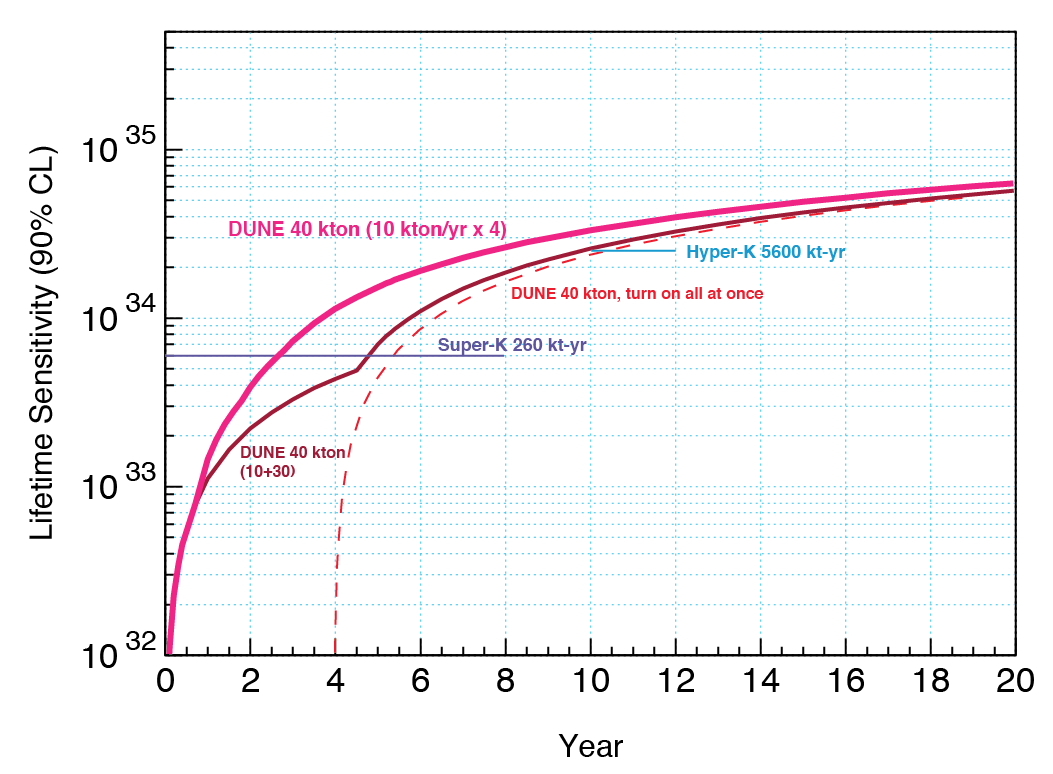
\includegraphics[width=0.7\textwidth]{figures/lar4x10.png}
\end{dunefigure}

Many models in which the $p\to K^+\overline{\nu}$ channel mode is
dominant, e.g., certain supersymmetric GUT models, also favor other
modes involving kaons in the final state, thus enabling a rich program
of searches for nucleon decay in the DUNE LArTPC detector.


%%%%%%%%%%%%%%%%%%%%%%%%%%%%%%%%%%%%%%%%%%%%%%%%%%%%%%%%%%%%%%%%%%%%%%%%%%%%%%%%%%
\section{Supernova-Neutrino Physics and Astrophysics}

The neutrinos from a core-collapse supernova are emitted in a burst of
a few tens of seconds duration, with about half the signal emitted in the first
second. The neutrino energies are mostly in the range 5--50 MeV, and the
luminosity is divided roughly equally between the three known neutrino
flavors.  Current experiments are sensitive primarily to
electron antineutrinos ($\bar{\nu}_e$), with detection through the inverse-beta decay
process on free protons\footnote{This refers to neutrino interactions with the nucleus of a
hydrogen atom in H$_2$O in water detectors or in hydrocarbon chains in 
liquid scintillator detectors.},
 which dominates the interaction rate in water
and liquid-scintillator detectors.  Liquid argon has a unique sensitivity to
the electron-neutrino ($\nu_e$) component of the flux, via the absorption
interaction on $^{40}$Ar,
\begin{eqnarray*}
\nu_e +{}^{40}{\rm Ar} & \rightarrow & e^-+{}^{40}{\rm K^*}.
\end{eqnarray*} 
This interaction can be tagged via the coincidence of the emitted
electron and the accompanying photon cascade from the $^{40}{\rm K^*}$
de-excitation.  About \num{3000} events would be expected in a \ktadj{40}
fiducial mass liquid argon detector for a supernova at a distance of
\SI{10}{\kilo\parsec}.  In the neutrino channel the oscillation
features are in general more pronounced, since the $\nu_e$ spectrum is
always significantly different from the $\nu_\mu$ ($\nu_\tau$) spectrum 
in the initial core-collapse stages, to a larger degree than is the
case for the corresponding $\bar{\nu}_e$ spectrum.  Detection of a large
neutrino signal in DUNE would help provide critical information on key
astrophysical phenomena such as
\begin{itemize}
\item the neutronization burst,
\item formation of a black hole,
\item shock wave effects,
\item shock instability oscillations, and
\item turbulence effects.
\end{itemize}


%%%%%%%%%%%%%%%%%%%%%%%%%%%%%%%%%
\subsection{Other Precision Neutrino Oscillation measurements}
\label{sec:exec-summ-physics-other}


%%%%%%%%%%%%%%%%%%%%%%%%%%%%%%%%%%%%%%%%%%%%%%%%%%%%%%%%%%%%%%%%%%%%%%%%%%%%%%%%%%
%\section{Precision Measurements with the DUNE Near Detector}
%This was section title in CDR

The DUNE near detector
will provide precision measurements of
neutrino interactions that are essential
for controlling the systematic uncertainties in the long-baseline
oscillation physics program.  The near detector 
will include argon targets and will measure the absolute flux and energy-dependent
shape of all four neutrino species, \numu, \anumu, \nue and \anue,
to accurately predict for each species the
far/near flux ratio as a function of energy.  It will also measure the
four-momenta of secondary hadrons, such as charged and neutral mesons,
produced in the neutral- and charged-current interactions that
constitute the dominant backgrounds to the oscillation signals.

The near detector will also be the source of data for a rich program
of neutrino-interaction physics in its own right. For an integrated
beam intensity of \num{1e20} 
protons-on-target at \SI{120}{GeV}, the expected number of events per
ton is \num{170000} (\num{59000}) 
\numu (\anumu) charged-current and \num{60000} (\num{25000}) neutral-current interactions in the $\nu$ ($\overline\nu$) beam\footnote{With PIP-II, the integrated protons-on-target per year is
  expected to be around $1.1\times 10^{21}$ at \SI{120}\GeV. The mass
  of the Ar target in the DUNE ND is expected to be approximately
  100~kg.}. 
  These numbers correspond to \num{e5} neutrino interactions
on argon per year for the range of beam configurations and near detector
designs under consideration.  Measurement of fluxes, cross sections
and particle production over a large energy range of
\SIrange{0.5}{50}{\GeV} are the key elements of this program.  These
data will also help constrain backgrounds to proton-decay signals
from atmospheric neutrinos.  Furthermore, very large samples of events
will be amenable to precision reconstruction and analysis, and will be
exploited for sensitive studies of electroweak physics and nucleon
structure, as well as for searches for new physics in unexplored
regions, such as heavy sterile neutrinos, high-$\Delta m^2$
oscillations, and light Dark Matter particles. %, and so on.

%%%%%%%%%%%%%%%%%%%%%%%%%%%%%%%%%%%%%%%%%%%%%%%%%%%%%%%%%%%%%%%%%%%%%%%%%
\section{Summary}

\fixme{No summary was specified in TP; this comes from CDR}

In summary, the primary science goals of DUNE are drivers for the
advancement of particle physics. The questions being addressed are of
wide-ranging consequence: the origin of flavor and the generation
structure of the fermions, 
he physical mechanism that provides the CP
violation needed to generate the baryon asymmetry of the universe, 
and the high-energy physics that would lead to the instability
of matter.  Achieving these goals requires a dedicated, ambitious and
long-term program.  No other proposed long-baseline neutrino
oscillation program with the scientific scope and sensitivity of DUNE
is as advanced in terms of engineering development and project
planning.  The staged implementation of
the far detector as four 10-kt modules will enable
exciting physics in the intermediate term, including a definitive mass
hierarchy determination and possibly a measurement of the CP phase, 
while providing the fastest route toward achieving the
full range of DUNE's science objectives.  Should DUNE find that the CP
phase is not zero or $\pi$, it will have found strong indications
($>3\sigma$) of leptonic CP violation.

The DUNE experiment is a world-leading international physics
experiment, bringing together the 
international neutrino community as well as leading experts in nucleon decay
and particle astrophysics to explore key questions at the forefront of
particle physics and astrophysics. The highly capable beam and
detectors will enable a large suite of new physics measurements with
potentially groundbreaking discoveries.




\fixme{1 page, mostly sensitivities}


%%%%%%%%%%%%%%%%%%%%%%%%%%%%%%%%%%%%%%%%%%%%%%%%%%%%%%%%%%%%%%%%%%%%
\section{Proton decay and the GeV scale non-accelerator physics program}
%\section{Nucleon Decay}
\label{sec:exec-summ-physics-pdk}

\fixme{2 pages}


%%%%%%%%%%%%%%%%%%%%%%%%%%%%%%%%%%%%%%%%%%%%%%%%%%%%%%%%%%%%%%%%%%%%
\section{Supernova neutrino burst and physics with low-energy neutrinos}
\label{sec:exec-summ-physics-sn-le}

\fixme{2 pages}


%%%%%%%%%%%%%%%%%%%%%%%%%%%%%%%%%%%%%%%%%%%%%%%%%%%%%%%%%%%%%%%%%%%%
\section{Precision physics with the near detectors}
%\section{Auxiliary Physics Program}
\label{sec:exec-summ-physics-nd}

\fixme{2 pages}

%%%%%%%%%%%%%%%%%%%%%%%%%%%%%%%%%%%%%%%%%%%%%%%%%%%%%%%%%%%%%%%%%%%%
%\subsection{Going Beyond the Standard Model}
%\label{sec:exec-summ-physics-bsm}
\section{Additional opportunities for Beyond Standard Model Physics}
%\section{Auxiliary Physics Program}
\label{sec:exec-summ-physics-aux}



\fixme{2 pages, make case that DUNE is best/unique, high level}



